\documentclass[jou,a4paper,notxfonts]{apa}
\usepackage{graphicx} 
\usepackage{palatino}
\usepackage{fancyhdr}
\pagestyle{fancy}

% header on first page
\fancypagestyle{plain}{%
\fancyhf{} % clear all header and footer fields
\fancyhead[L]{\small
Journal of Eye Movement Research\\
1(1):1, 1-2}
\fancyfoot[C]{\thepage}
\renewcommand{\headrulewidth}{0pt}
\renewcommand{\footrulewidth}{0pt}}

\title{Distributed Eye Tracking Network for Conveying Population Gaze in a Mobile Telepresence Scenario} %Fill this in

%please refer to http://www.ilsp.gr/homepages/protopapas/apacls.html#titlhead for different numbers of authors and affiliations
\threeauthors{First Author}{Second Author}{Third Author}
\threeaffiliations{First affiliation}{Second Affiliation}{Third Affiliation}


\journal{}
\volume{}

\abstract{Mobile telepresence technology allows one or several remote users to visit a distant geographical space using
a mobile robot. The robot can carry a 360$^\circ$ panoramic camera that provides to the remote users an immersive
viewing perspective of the robot environment . One limitation of this technology is that for humans around the robot or
elsewhere, is difficult to gather a sense of where in the robot's environment the remote users are paying attention to.
Here, we propose the usage of a distributed network of low cost eye trackers to monitor the gaze behavior and field of
view of the remote users within the panoramic video live streamed by the robot. The system transmits the gaze data of
the remote users to the robot that then superimposes the aggregated gaze behavior of the remote users in a condensed 2D
representation of the panoramic image it is currently capturing from the environment. We use as an illustrative
application, a robot being employed to visit a museum virtually by several high school students distributed across
remote locations in Australia. A human  museum guide, directs the robot around the museum while explaining and
interacting with the remote students through the visual display on the robot. The visualization of the gaze
behavior of the remote students in real time provides a useful feedback signal to the museum tour guide about where the
remote students are paying attention to so the guide can adapt his behavior accordingly.

\linebreak
\linebreak
{\bf Keywords: eye tracking, gaze tracking, telepresence, eye tracking network, gaze aware interfaces, pervasive
computing, HCI, gaze responsive interfaces, human computer interaction}}

\acknowledgements{}
\shorttitle{}
\rightheader{}

% repeat the authors here (use et al if more than three authors):
\leftheader{ }

\begin{document}

%-------------------------------------
\maketitle


\lhead{\small
Journal of Eye Movement Research\\
1(1):1, 1-2
}
\rhead{
Author, A., Author, B., & Author, C. (2007)\\
Short Title
}
\thispagestyle{plain}

\section{Introduction} 
Telepresence technology allows a person to feel or to have an effect as if they were present at a place other than their
real location. Telepresence technology requires that the user is provided with sensory stimuli conveying information
about the remote location in order to re-create the feeling of being in that other location. Users can be given the
option of interacting with the remote location through output effectors. This can be achieved by sensing, transmitting
and duplicating in the remote location the user's position, movements, actions, or voice. Hence, in realistic
telepresence sytems, information flows in both directions between the user and the remote location.
Telepresence systems enable collaboration independent of location and provide considerable cost savings for numerous
scenarios. A robotic telepresence can allow a subject to move virtually through a distant building by remotely
controlling a wheeled robot equipped with a camera, microphone, loudspeaker and screen that can optionally display live
video of the subject�s face. Telepresence systems possibilities have increase considerably in the last years thanks to
advances in robotics and telecommunications.


In this work with present a telepresence systems that allows remote visitors to visit a museum using a semi autonomous
mobile robot and an immersive web interface. The system is designed to allow remote visitors to feel as they are on an
actual tour in the museum. The innovative part of the system, is that a network of eye trackers monitors the gaze
behavior of the museum visitors and transmits the gaze data to the mobile robot that displays it in order to provide to
the educator at the museum with information about what is attracting the gaze (and hence the attention) of the remote
students.


The point of regard (PoR) of a computer user on the screen can be estimated using video oculography gaze tracking. The
usage of eye gaze as a pointing or control mechanism is well documented in the literature \cite{duchowski,Rozado2012,
Bonino2011, danhansenrevieweyetrackingmethods}. However, the accuracy limitations of gaze estimation algorithms to
determine the precise coordinates of a user's gaze on the screen offsets the advantages of using the eyes as a pointing
mechanism and this has prevented the widespread adoption of gaze tracking as a substitute of the mouse
\cite{Rozado2012a, giaet, myiwann2011}. Gaze tracking has found a niche application to study how computer users interact
with content on a computer screen. The gaze data accumulated during a gaze tracking session can be visualized off-line
as a heat map data structure. A heat map captures the accumulated degree of attention that a given user places at
different points on the screen during the gaze tracking trial. Hence, it is well-established that the direction of gaze
reflects the user's focus of attention on the screen \cite{Zhai2003}, and hence, it provides a hint about intention.
In this work, we propose the usage of the network of eye trackers to convey the gaze behavior of virtual
museum visitors in a remote telepresence systems.


% Literature review
The concept of telepresence systems is not new. The work from \cite{minsky1980telepresence} coined the term
\emph{telepresence} to describe systems that would transform work, manufacturing, energy production and medicine. Minsky
proposed the idea of being able to work in another country or planet through remote presence.

One of the first and most popular applications of the presence is videoconferencing \cite{duncanson1973video}. The
review  from \cite{Egido:1988:VCT:62266.62268} highlighted some of the limitations of the technology at the time, most of which have
already been overcome.

Another branch of telepresence that has gathered a lot of attention in the research literature is telesurgery
(``surgery at a distance'') \cite{green1995telepresence}, a technique that allows surgeons to operate robotically on a
patient that is located in a different geographical point. It has the potential to revolutionize healthcare delivery by bringing healthcare to
previously inaccessible settings \cite{holt2004telesurgery}.


More recently, telepresence robots that are controlled remotely and the Palau human to explore these kind your graphical
location have been proposed \cite{schultz1991telepresence} and have received a considerable amount of attention
\cite{tsui2011exploring}.


An important feature of robotic telepresence systems is the ability to capture their surrounding environment in order to
convey a realistic representation  of it to the remote user. Panoramic images are a key component of many modern Robotic
telepresence systems in North third to provide the function of transmitting a visual representation of the robot's
surrounding environment. The work from \cite{Gledhill2003435} provides a good overview of panoramic imaging summarizing
and comparing some of the methods to carry out capturing, image processing, image stitching, 3-D reconstruction,
rendering and visualization.


Gaze tracking has been used extensively to monitor the gaze behavior of subjects in a variety of circumstances and
environments \cite{duchowski, jacob2003eye, myiwann2011}. However, to our knowledge, there is no literature available on
the utility of using gaze tracking to transmit the gaze behavior of remote users in a telepresence system. The amount of
literature on using networks of eye trackers is also very limited due to their high cost of the devices until very
recently.

%-----------------------------
In Summary, the mobile telepresence system that we present here allows live interaction between remote students and an
educator in the museum.  Multiple remote students connect via a single robot, but control their own view within the
gallery. Remote students can access additional digital content about objects on display augmenting the tour experience.
A network of eye trackers in the remote students' computers monitor and transmit their gaze behavior. This gaze behavior
data is displayed in the robot screen to provide feedback signal to museum tour guide about where students are paying
attention to. This information closes the interaction loop between the educator in the museum and the remote students
and offsets some of the nonverbal communication limitations of telepresence systems by signaling to the museum tour
guide where the remote museum visitors are paying attention to at any given instant in time.


%XXXXXXXXXXXXXXXXXXXXXXXXXXXXXXXXXXXXXXXXXXXXXX
\section{Method}

\subsubsection{Eye-tracking system}
Eyes are used by humans to obtain information about the surroundings and to communicate information. When something
attracts our attention, we position our gaze on it, thus performing a \textit{fixation}. A fixation usually has a
duration of at least 150 milliseconds (ms). The fast eye movements that occur between fixations are known as
\textit{saccades}, and they are used to reposition the eye so that the object of interest is projected onto the fovea.
The direction of gaze thus reflects the focus of \textit{attention} and also provides an indirect hint for
\textit{intention} \cite{velichkovsky}.


A video-based gaze tracking system seeks to find where a person is looking, i.e. the Point of Regard (PoR), using images
obtained from the eye by one or more cameras. Most systems employ infrared illumination that is invisible to the human
eye and hence it is not distracting for the user. Infrared light improves image contrast and produces a reflection on
the cornea, known as corneal reflection or glint. Eye features such as the corneal reflections and the center of the
pupil/iris can be used to estimate the PoR. Figure \ref{screenGazeTracker} shows a screenshot of an eye being tracked by
the open-source ITU Gaze Tracker \cite{lowcostitugazetracker,Rozado2012}. In this case, the center of the pupil and two
corneal reflections are the features being tracked.


\begin{figure}[tp]
 %\fitbitmap[scale=0.5]{figures/screenGazeTracker.jpg}
 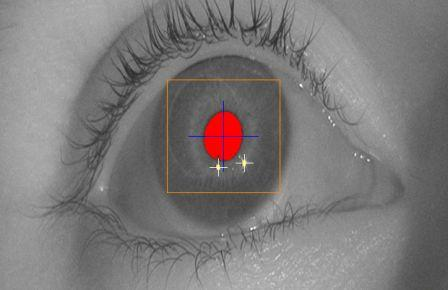
\includegraphics[width=0.5\textwidth, height=40mm]{figures/screenGazeTracker.jpg}
 \caption{\textbf{The Open Source ITU Gaze Tracker Tracking One Eye.} The
  features tracked in the image are the pupil center and two corneal reflections. These features are used by the gaze 
  estimation algorithms to determinine the PoR of the user on the screen.}
 \label{screenGazeTracker}
\end{figure}

In most eye tracking studies, the PoR of the user is employed as a pointing device that substitutes the mouse. For this
work, eye tracking was used behind the scenes just to capture gaze behavior and transmit it to the robot in order for
it to display the aggregated gaze behavior of several users to the museum educator. 

A set of 3 Tobii Rex eye trackers and 1 Tobii X1 light eye tracker was used in the experimental part. Both systems
track gaze at 30 frames per second (fps) with an average gaze estimation accuracy of 0.5 degrees at 60cm from the screen, 
\cite{TobiiTechnologyAB}. A simple exponential smoothing filter, \cite{Kumar2007}, of the raw gaze tracking data was
carried out to prevent jitter.


\subsection{Robot}
% Fred, maybe you could provide more specific and technical details about this part?
We use a commercial robot that carries a head-height omnidirectional camera and a display screen, see
Figure \ref{MuseumRobot}. the robot also carries a forward-looking camera and X onboard computers and Wiffi antennas.

\begin{figure}[tp]
 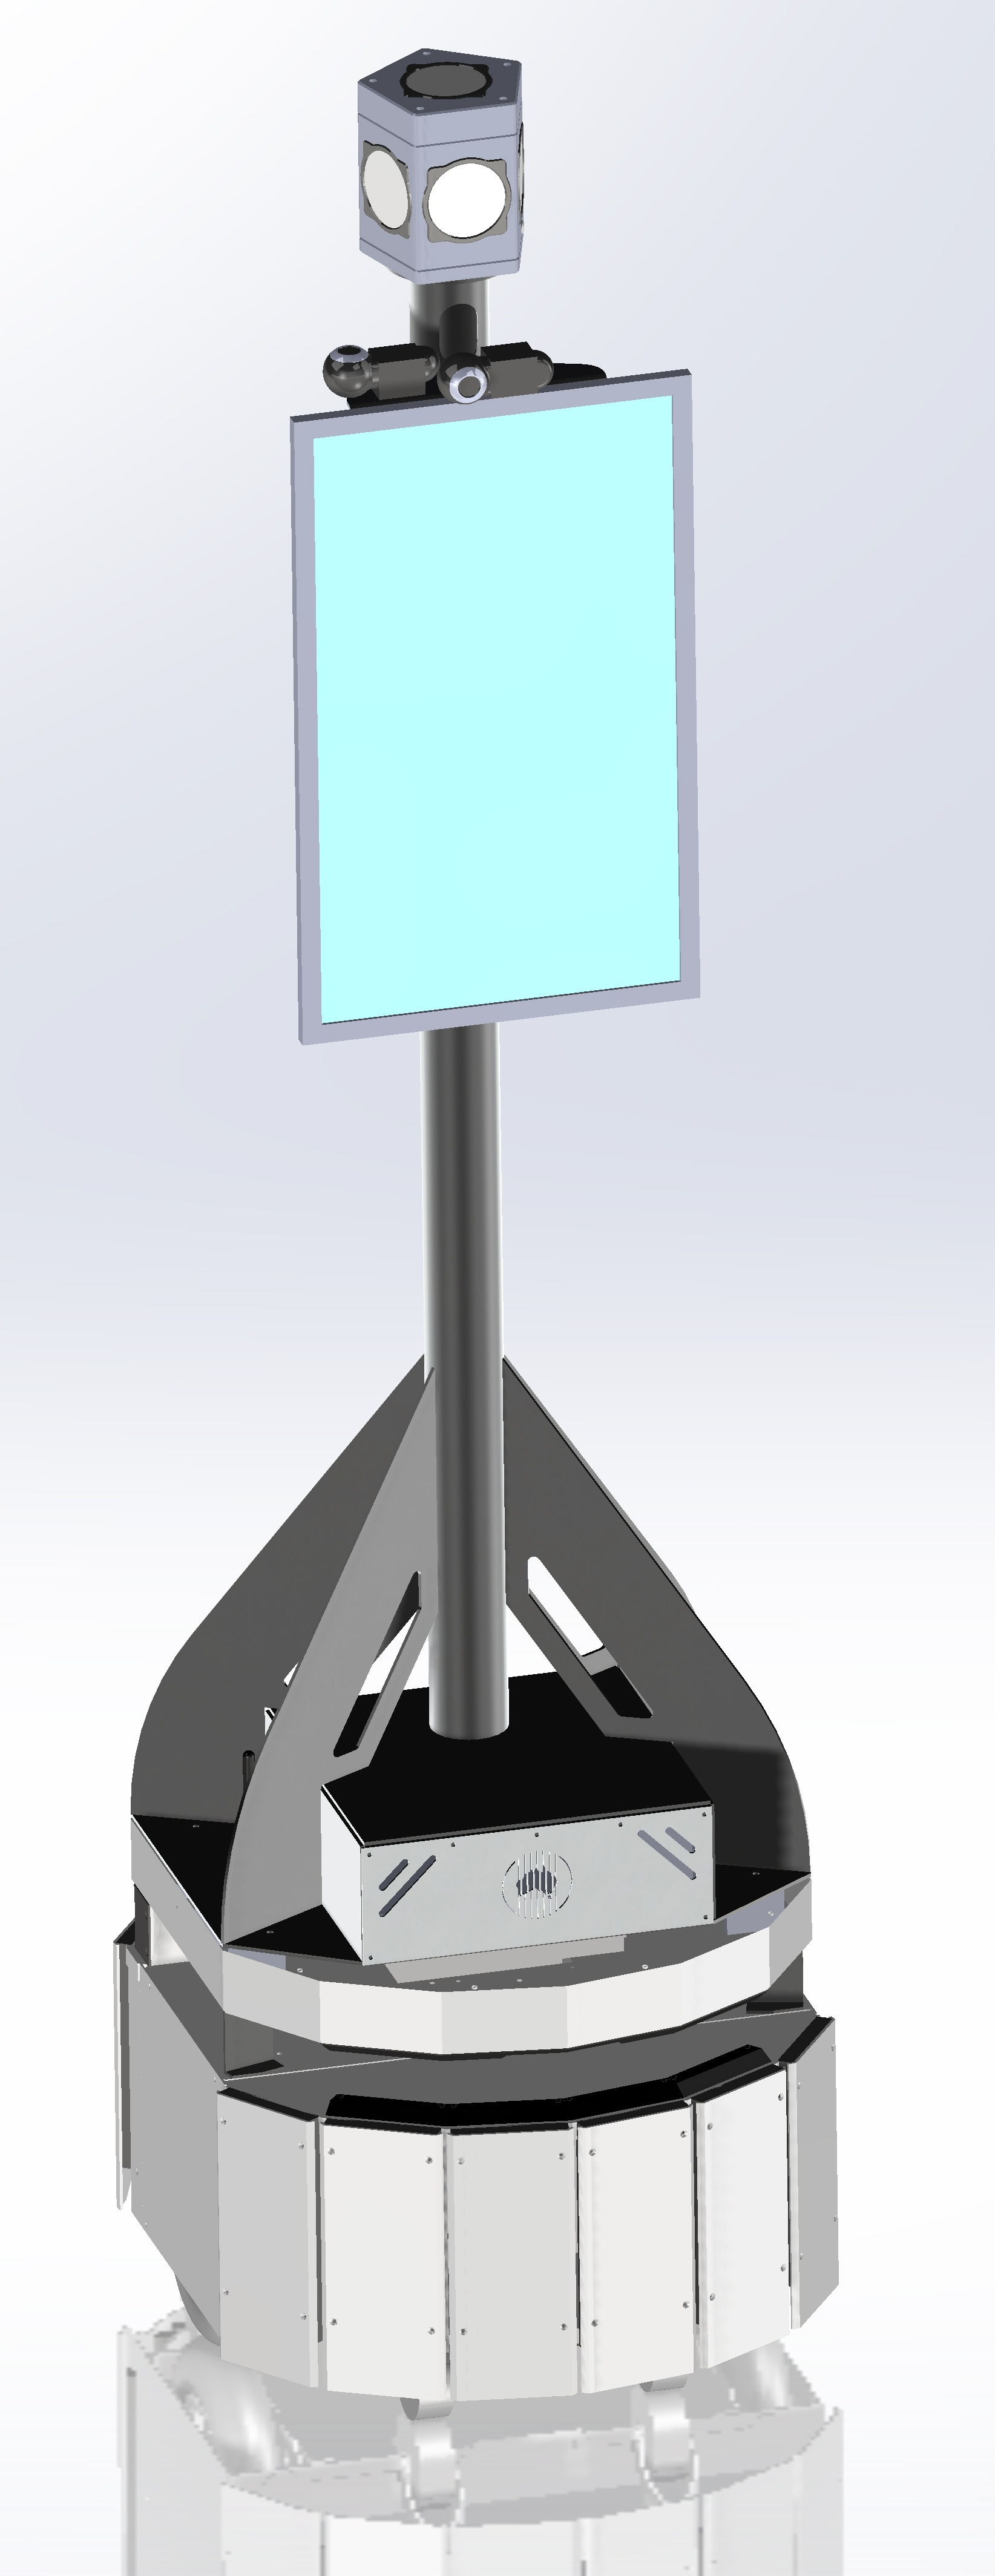
\includegraphics[width=0.3\textwidth, height=60mm]{figures/MuseumRobot.jpg}
 %\fitbitmap{figures/ladybug.jpg}
 \caption{Prototype of telepresence robot}
 \label{MuseumRobot}
\end{figure}

The robot moves at walking speed within any wheelchair accessible space. The robot is able to navigate to different
locations in the museum under the supervision of the tour guide. Using light depiction and ranging technology, the robot
is able to detect walls, exhibits and people around. Hence, the robot can monitor its location in space and to map its
surroundings into a real-time map of the gallery space. The robot's navigation system also includes  a dynamic obstacle
avoidance system.



\subsection{Museum Tour Guide}
The teacher wears a wireless lapel microphone, to ensure that he can be heard by the remote students. The museum tour 
guide can see who is online and which students have questions via the display on the front of the robot.

\subsection{360$^\circ$ Video and panoramic viewer}
A panorama is a single wide-angle image of the environment around the camera \cite{Gledhill2003435}. The most realistic
types surround the camera on the horizontal plane (360$^\circ$), and 180$^\circ$ in the vertical field of view. 
There are different ways to capture panorama: single, rotated about its optical center, single omnidirectional camera (
using multiple cameras facing  in different directions) or using a stereo panoramic camera from which started
information can be extracted.

Several cameras capture multiple images of a scene from different viewpoints from which stereo information can be
calculated and then used to create a 3-D model of the scene.

The 360$^\circ$  panoramic camera (Figure \ref{ladybug}) used in our telepresence system was mounted on top of the robot
and streamed a high-resolution omnidirectional image to the remote students. Each remote students can then 
independently ``look around'' the gallery using the panoramic viewer within their browser, see Figure \ref{omnidirectionalimage}.


\begin{figure}[tp]
 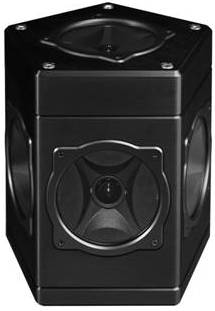
\includegraphics[width=0.3\textwidth, height=60mm]{figures/ladybug.jpg}
 %\fitbitmap{figures/ladybug.jpg}
 \caption{An image displaying the 360$^\circ$ panoramic camera on top of the robot}
 \label{ladybug}
\end{figure}


\begin{figure}[tp]
 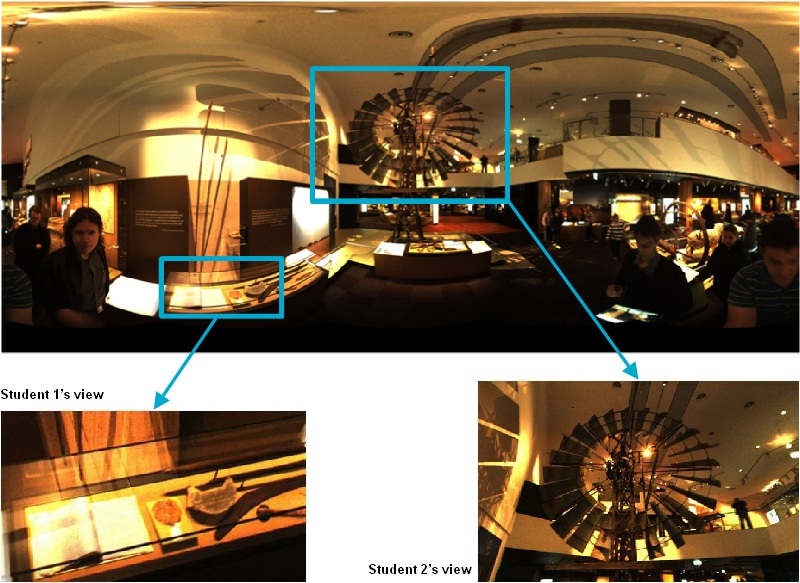
\includegraphics[width=0.3\textwidth, height=60mm]{figures/omnidirectionalimage.jpg}
 %\fitbitmap{figures/ladybug.jpg}
 \caption{Images from the 360$^\circ$ camera on top of the robot are combined to form a high-resolution omnidirectional
 image.}
 \label{omnidirectionalimage}
\end{figure}


\subsection{Remote Students' Computers}
Each student computer is equipped with a low cost eye tracker capturing frames at 30Hz. The students focus of attention
in the panoramic viewer is recorded. This includes the horizontal and vertical field of views (that determine the plane
being displayed on screen at any given time) and the x, y coordinate of their gaze on screen. This for parameters define
the point in 3D space the student is looking at. This aggregated data is sent back to the robot, that converts it to a
3D point in space.

Images from the 360 degree camera on top of the robot are combined to form a high-resolution omni-directional image,
see Figure \ref{ladybug}, and the points of regard of several students are projected into this image to provide feedback
to the educator about where the students are paying attention to in the scene, see Figure \ref{aggregatedGazeBehavior}
and \ref{robotDisplay}.

\begin{figure}[tp]
 \fitbitmap{figures/museumtourview.jpg}
 \caption{Remote interface client through which student can look around the
museum with freedom to look at different areas within the 360 field of view environment}
 \label{museumtourview}
\end{figure}

\begin{figure}[tp]
 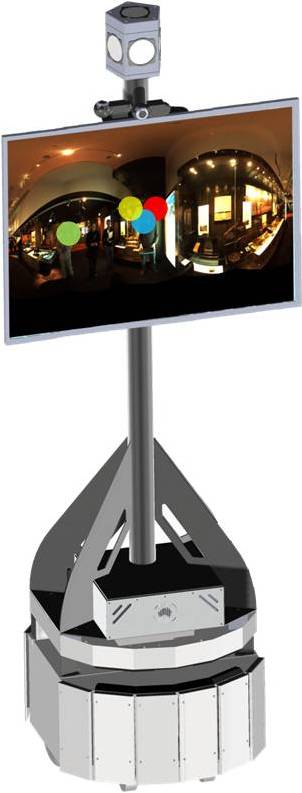
\includegraphics[width=0.4\textwidth, height=140mm]{figures/robotDisplay.jpg}
 \caption{Aggregated gaze behavior of remote
students superimposed into the omni-directional is shown in the robot display so the tour guide for instance can obtain
feedback about what areas in space the remote students are paying attention to}
 \label{robotDisplay}
\end{figure}

The user studies to be carried out in the future will involved students (ages 10-16) from several national high schools.
Their gaze will be monitored through a network of low cost Tobii Rex eye trackers. These eye trackers offer a
resolution of 30 samples per second and produce gaze estimation with an average accuracy of 0.5 degrees at 60
cm from the screen. 


The eye trackers are connected through a network. The TCP protocol is used to issue commands to the eye trackers
such as start calibration, calculate results from calibration, start tracking, stop tracking. Gaze estimation is
sent through the UDP protocol, since the system can afford to lose some packets. 

The krpano panoramic viewer is used by the students to freely move within the 360$^\circ$ video stream. Javascript
scripts are used to gathered the horizontal and vertical field of view coordinates of each student through the panoramic 
image.

\begin{figure}[tp]
 \fitbitmap{figures/aggregatedGazeBehavior.jpg}
 \caption{Network of eye trackers on the remote students computer captures the gaze behavior of the students and
 combines the gaze data into a high-resolution omni-directional image}
 \label{aggregatedGazeBehavior}
\end{figure}


%---------------------------------------------------------------
\section{Application}

Bla bla bla
Video demo: \url{}

\section{Discussion}

National institutions such as museums have a responsibility to reach regional and remote school students who are often
unable to visit them physically due to factors such as cost and distance. A mobile telepresence system provides an
opportunity for regional and remote students to participate in visits to museums and other educationally relevant
institutions.


A key challenge for telepresence systems will how to leverage the new opportunities provided by telepresence
technology to engage students and stimulate learning.

The interactive nature of the systems permits interactive learning rather than passive and collaborative learning by
allowing students to interact with each other and with the tour guide.


System is immersive, ( remote students feel as if they are present in the gallery )
interactive ( remote students engage in discussions with the educator and other students on the tour )
Engaging ( students can explore digital content that is relevant to the current conversation)

Telepresence facilitates one region of the world exporting specialized skills to anywhere

Elimination of many chemical and physical health hazards

Reduction of transportation costs and of energy and commuting time

Importance of high quality sensory feedback

Time and cost benefits. The visual aspect greatly enhances communications, allowing for perceptions of facial
expressions and other body language.

\bibliography{library}
\end{document}

